\chapter{Refining the bounds}
\label{chap:bounds}

In previous chapters we have established that $\gdist(p)$ is asymptotically logarithmic, or, more precisely, that
\begin{align}
	2.73 \approx 3 \log_3(e) < \frac{\gdist(p)}{\log(p)} < 5 \log_2(e) \approx 7.21
\end{align}
for all primes $p$. The obvious question is -- what are the best possible constants in these estimates?

While the question is open, in this chapter we provide evidence which suggests that the following might be true:

\begin{conj}
\label{conj:lim-gdist}
Let $P$ be a real such that $P^3=P+1$. Then for primes $p$:
\begin{align}
	\lim_{p \rightarrow \infty} \frac{\gdist(p)}{\log(p)} = 1/\log(P) \approx 3.56.
\end{align}
\end{conj}%

Our argument is based on the connection of $\gdist(p)$ to dissections of triangles. Recall that the key to establish the upper bound was the fact that $\gdist(p) \leq t(p)$. However, it seems that the following conjecture might be true:

\begin{conj}
\label{conj:gdistp-equals-tp}
Let $p$ be a prime. Then $\gdist(p) = t(p)$.
\end{conj}%

If that was the case, we could find bounds of $\gdist(n)$ by examining triangle dissections only. In this chapter we present computational data of Rosendorf \cite{Rosendorf04} and of our own which support the following:

\begin{conj}
\label{conj:lim-hat-tn}
Let $P$ be a real such that $P^3=P+1$. Then
\begin{align}
	\lim_{n \rightarrow \infty} \frac{\hat t(n)}{\log(n)} = 1/\log(P).
\end{align}
\end{conj}%

Note that Conjectures \ref{conj:lim-hat-tn} and \ref{conj:gdistp-equals-tp} imply Conjecture \ref{conj:lim-gdist}.

In some sense, as we will see, it is easier to approach Conjecture \ref{conj:lim-hat-tn}. One of the reasons is that we do not have to restrict ourselves only to primes, but can regard all numbers equally.

%%%
%%%
%%%
\section{Padovan sequence}

\begin{defn}
\emph{Padovan sequence} is a linear recurring sequence $(a_k)_{k \geq 1}$ defined by
\cosyalign{
	a_1 = a_2 = a_3 = 1, \quad a_{k+3} = a_{k+1}+a_k \ \ \mbox{ for } n \geq 1.
}%
The first few terms are $1, 1, 1, 2, 2, 3, 4, 5, 7, 9, 12, 16,\dots$
\end{defn}

For more information about the sequence see e.g. \cite{OEIS}.

Let $P, \lambda_1, \lambda_2$ be roots of the polynomial $x^3-x-1$, where $P$ is the only real root. Then we can write explicitly
\cosyalign{
	a_k = c_0P^k + c_1\lambda_1^k + c_2 \lambda_2^k
}%
for some complex constants $c_0,c_1,c_2$. Enumerating the values, we get $|\lambda_1|, |\lambda_2| < 1$ and $c_0 \approx 0.545$ is a real. Therefore $a_k \sim c_0P^k$, or $\log_P(a_k) \sim k$.

The number $P \approx 1.325$ is called \emph{the plastic constant}. As a side note, along with its mathematical properties, it has also its application in architecture \cite{Stewart96}.

\begin{defn}
Let $n$ be a positive integer. By $\spb(n)$ we denote an integer such that
\cosyalign{
	a_{\spb(n)-1} < n \leq a_{\spb(n)}.
}
\end{defn}

Note that $a_{\spb(n)}$ is the nearest term in Padovan sequence which is larger or equals to $n$. Also $\spb(n) \sim \log_P(n)$.

Consider a trapezoid consisting of three unit triangles. In each step, we can attach a triangle to the longest side of the shape to get a pentagon. This way we get a spiral-like tiling. By adding two more triangles to the pentagon we obtain a $\circledast$-free dissection of a triangle. (Figures \ref{fig:spiral}, \ref{fig:spiral2}.)

\begin{figure}[htb]
\centering
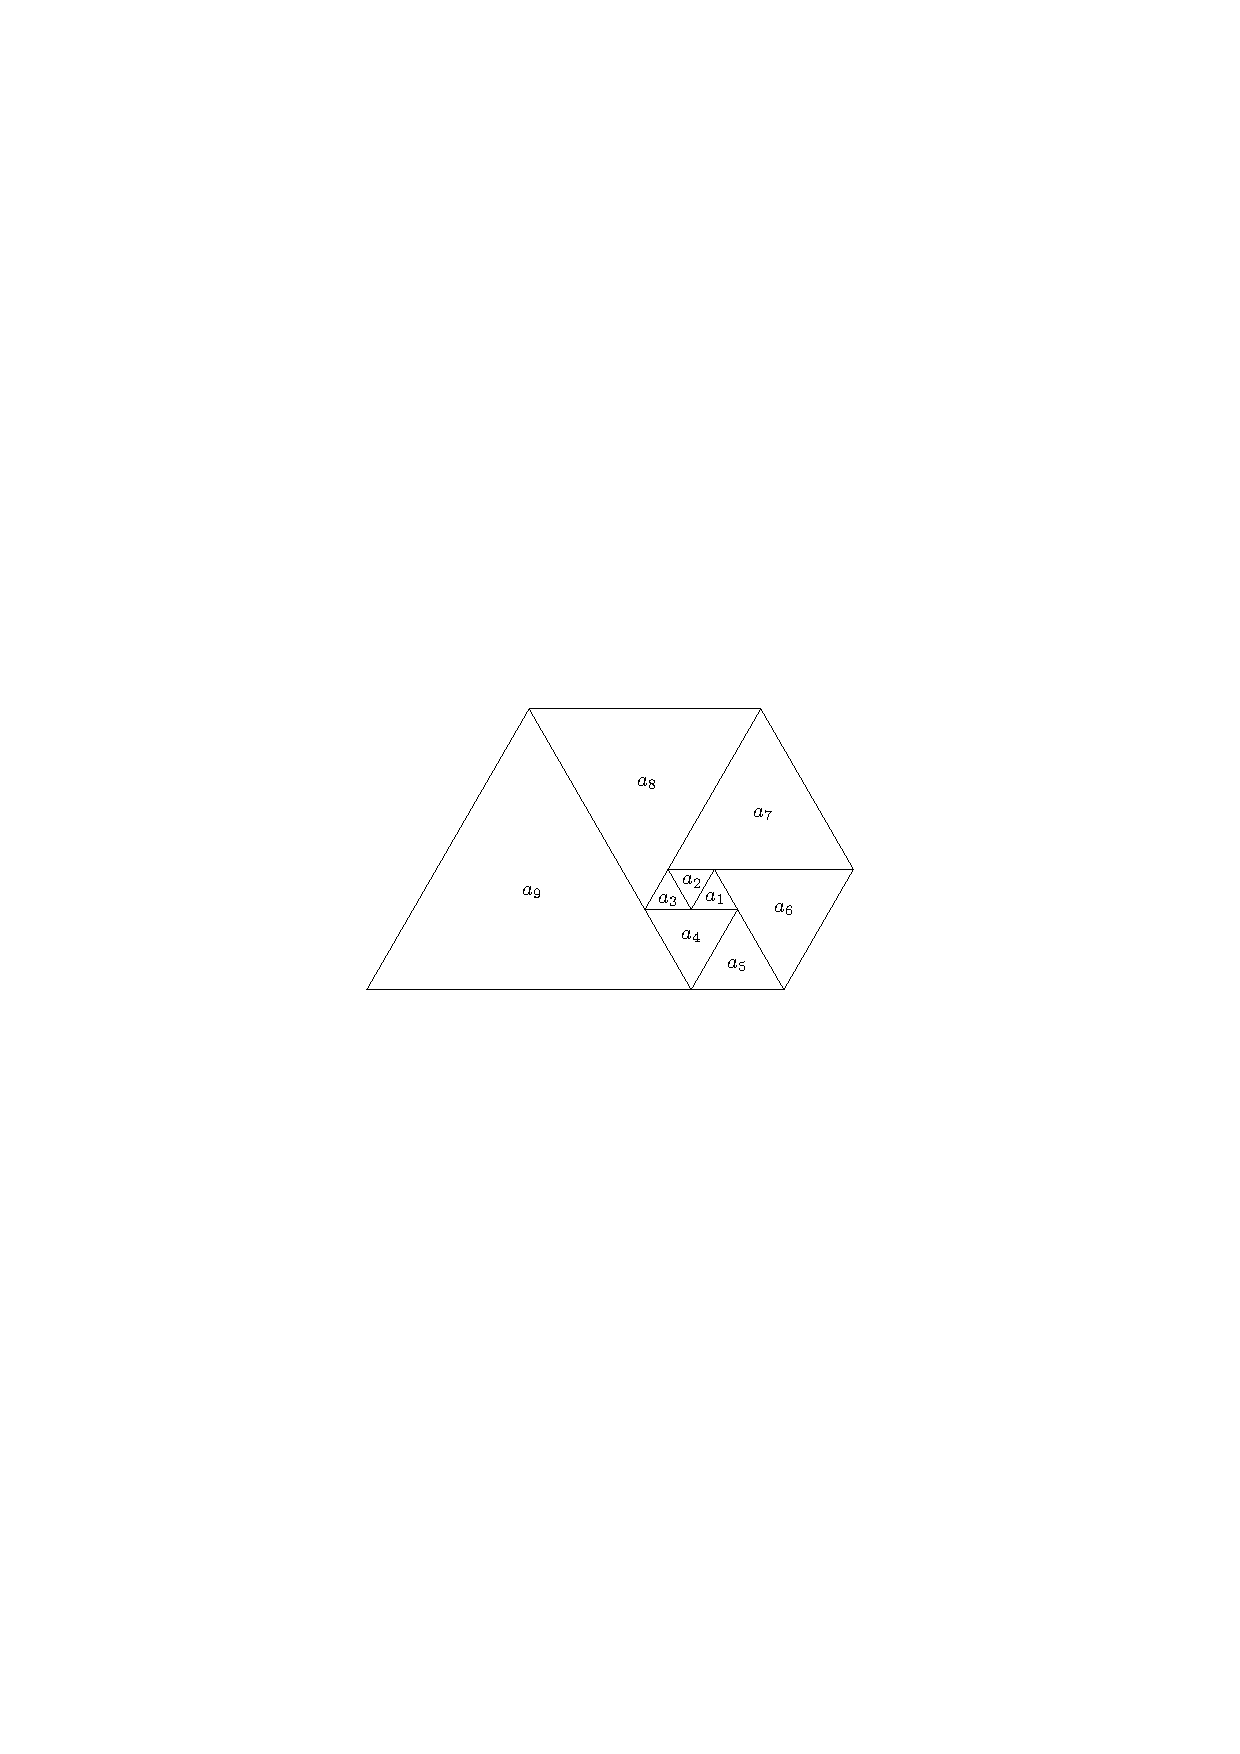
\includegraphics[width=0.6\textwidth]{img/spiral.pdf}
\caption{Spiral tiling.}
\label{fig:spiral}
\end{figure}

\begin{figure}[htb]
\centering
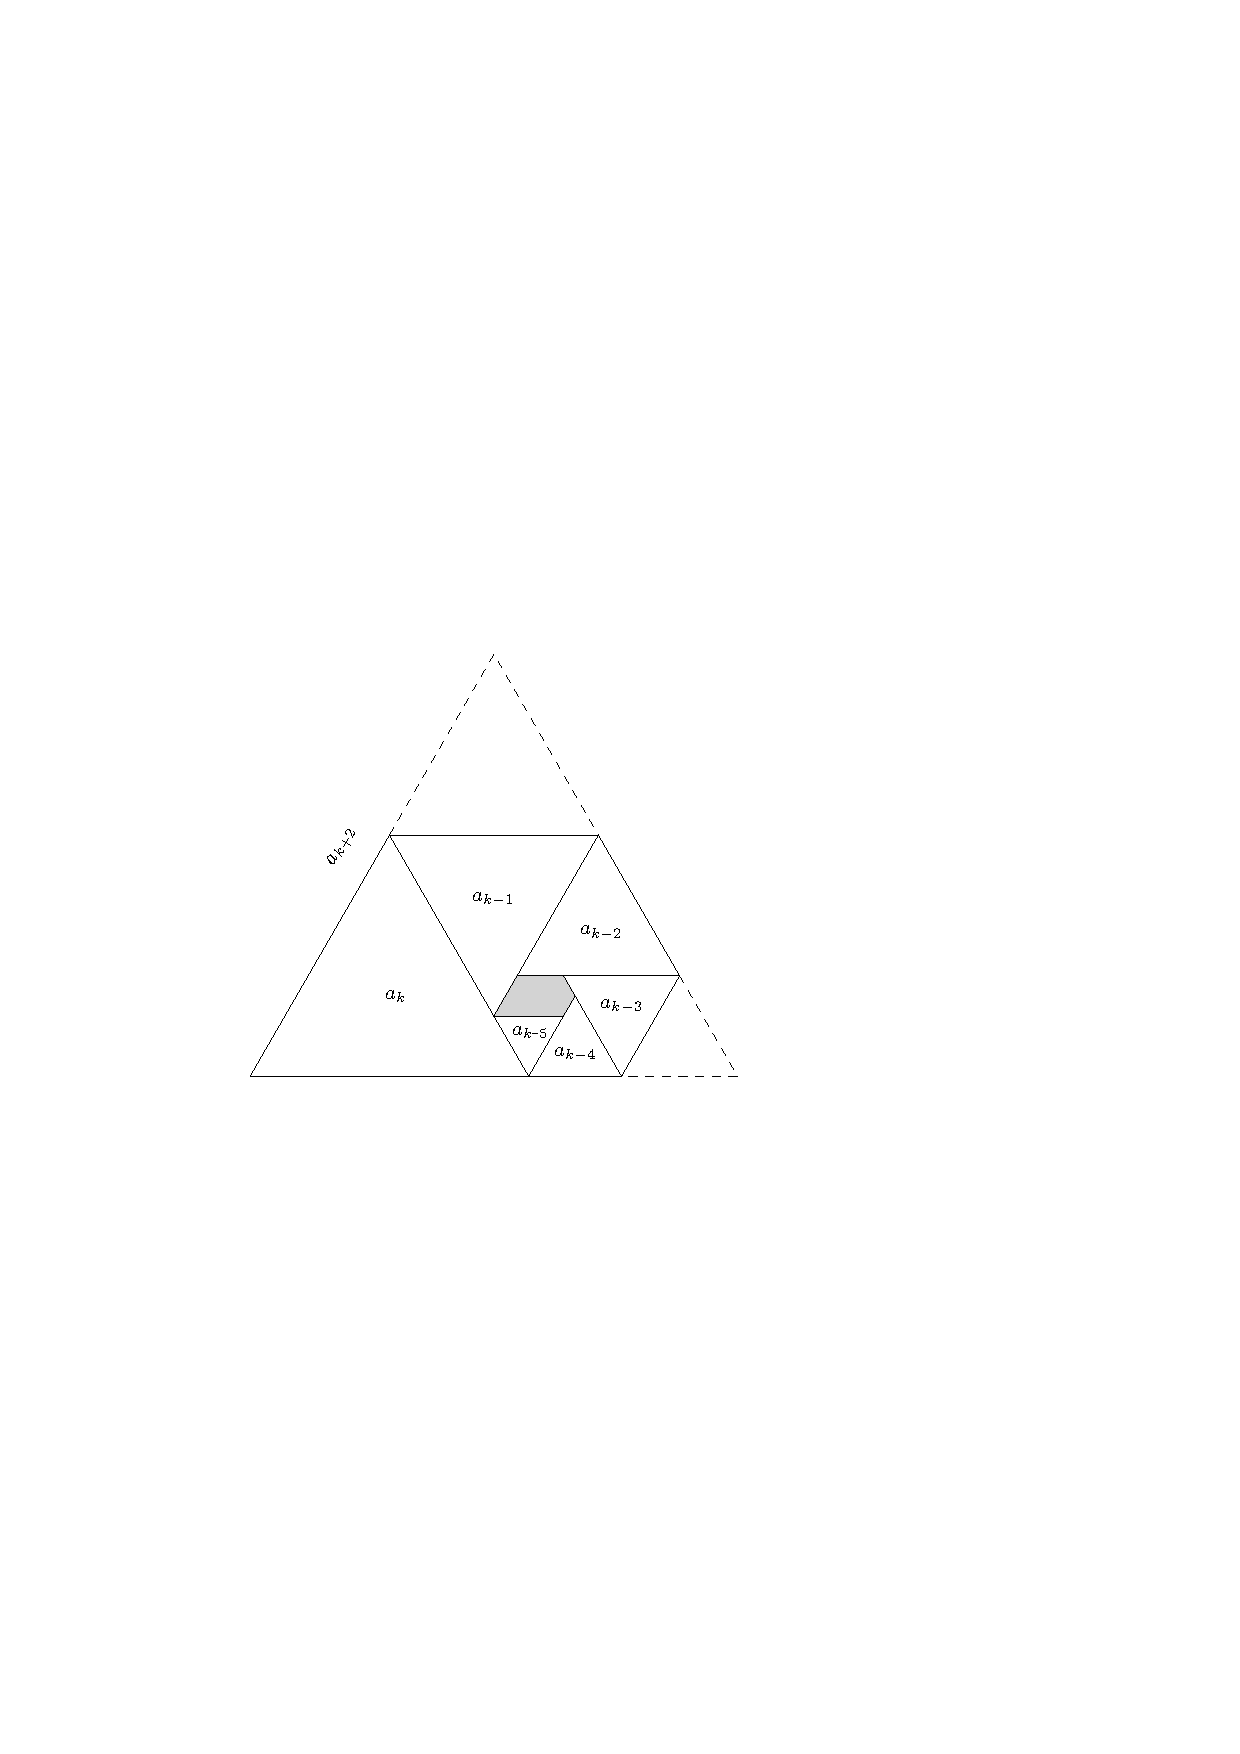
\includegraphics[width=0.6\textwidth]{img/spiral_triangle.pdf}
\caption{Completion of a pentagon into a triangle.}
\label{fig:spiral2}
\end{figure}

It is easy to derive that the sizes of the triangles are exactly the terms of Padovan sequence. Therefore we can construct a dissection of a triangle of side $a_{k+2}$ into $k+2$ triangles. Since in such a dissection there is always a triangle of side 1, we obtain
\cosyalign{
	\hat t(a_k) \leq k = \spb{a_k} \sim \log_P(a_k).
}%


%%%
%%%
%%%
\section{Computational results of Rosendorf}
Based on Drápal's suggestion, Rosendorf studied in his master's thesis \cite{Rosendorf04} a modification of the spiral tiling, which can be applied to triangles of any size. Consider the following algorithm:

\begin{alg} \ 
	\begin{cosyitemize}
		\item In the beginning, from two corners of the original triangle cut off two triangles to get a pentagon or a parallelogram;
		\item Then, until the remaining shape is a triangle, cut off a triangle from the current shape to get either a pentagon, a parallelogram, a trapezoid or a triangle.
	\end{cosyitemize}
\end{alg}%

The algorithm is nondeterministic -- if the current shape is not a pentagon, we can choose the placement and the size of the triangle to be cut off. Rosendorf proved that these dissections are exactly those which are $\circledast$-free and do not contain a subset of triangles forming a proper convex hexagon. Following his notation, let us denote such a dissection as \emph{(M6)}, standing for "missing hexagon".

Rosendorf enumerated all minimal (M6) dissections of triangles of side less than 10252. The data show that
\begin{align}
	\hat{t}(n) \leq \spb(n)+2 \qquad\hbox{for $n < 10252$.}
\end{align}

On the other hand, he also proved that at least $\spb(p)$ triangles are needed in an (M6) dissection of a triangle of prime side $p$. That, however, is not true when we allow all $\circledast$-free dissections.


%%%
%%%
%%%
\section{Enumerations of minimal dissections}

To support Conjecture \ref{conj:lim-hat-tn}, we generated all triangle dissections up to size 23 and thus established values of $t(n)$ and $\hat t(n)$ for $n \leq 416$. For comparison, in \cite{DrapalHamalainen10} Drápal and Hämäläinen were able to generate dissections up to size 20, which corresponds to $n \leq 160$. They were, however, interested in other properties of triangulations, not in the values of $t(n)$ and $\hat t(n)$.

\side{formulacia}
We use essentially the same algorithm as in \cite{DrapalHamalainen10}.\footnote{Although it is not absolutely clear from their paper, our implementation has probably better time complexity.} Separated connected spherical latin bitrades are equivalent to planar Eulerian triangulations (Theorem \ref{thm:connected-spherical-separated}). Planar Eulerian triangulations can be efficiently generated by Brinkmann and McKay's package \emph{plantri} \cite{BrinkmannMcKay99}. We will show an algorithm with which every triangle dissection can be reconstructed from a separated connected spherical latin bitrade.

\bigskip

Let $\D$ be a $\circledast$-free dissection of $\Delta_n$, and $(T^*, T^\vartriangle)$ an embedding of it into the plane $x+y+z=0$.

\begin{lem}
$(T^*, T^\vartriangle)$ is a connected spherical latin bitrade.
\end{lem}
\begin{proof}
It suffices to show that the graph of $(T^*, T^\vartriangle)$ is connected and planar. A formal proof can be found e.g. in Tutte \cite{Tutte48}, we give only an illustration of it on Figure \ref{fig:triangulation-graph}. Black vertices correspond to elements of $T^*$, white to elements of $T^\vartriangle$.

\begin{figure}[htb]
\centering
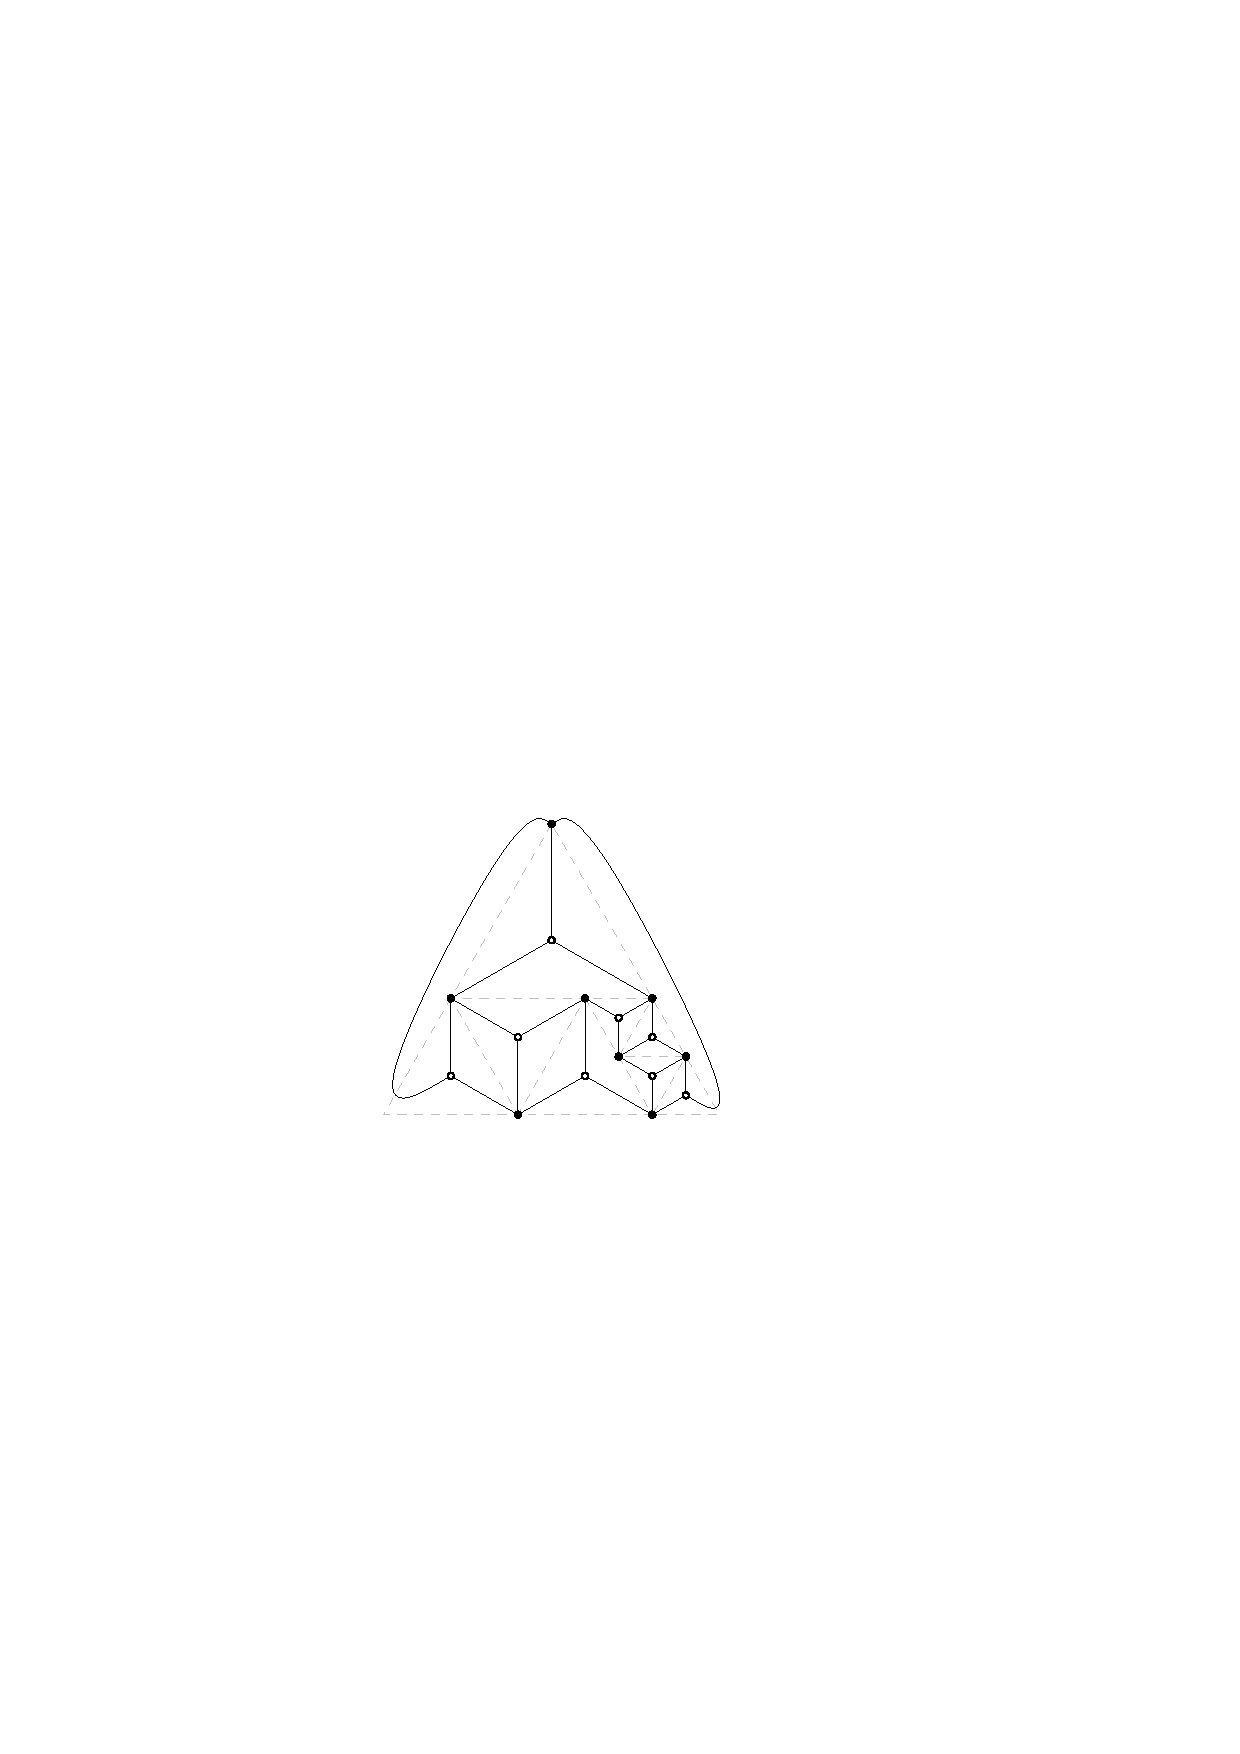
\includegraphics[width=0.5\textwidth]{img/triangulation_graph.pdf}
\caption{The graph obtained from a triangulation is connected and planar.}
\label{fig:triangulation-graph}
\end{figure}
\end{proof}

Let $(T,T')$ denote the separated latin bitrade obtained from $(T^*, T^\vartriangle)$ by the procedure described in Section \ref{sec:latin-bitrades}, and let $h:T \rightarrow T^*$ be the natural projection homotopy of $T$ onto $T^*$. Further denote $|T|$ and the support of $T$ such that:
\begin{itemize}
	\item $T = \{t_1, \dots, t_{|T|}\} \subset R \times C \times S$,
	\item $R = \{r_1,\dots,r_{|R|}\},\ 
		C = \{c_1,\dots,c_{|C|}\},\ 
		S = \{s_1,\dots,s_{|S|}\}$,
	\item $(r_1,c_1,s_1) \in T$,
	\item all elements of $X := R \cup C \cup S$ are used in $T$.
\end{itemize}%
Let $h = (h_R, h_C, h_S)$. Since $T^* \subset \Z \times \Z \times \Z$, we have
\cosyalign{
	h_R: R \rightarrow \Z,\ h_C: C \rightarrow \Z,\ h_S: S \rightarrow \Z.
}%
Because embeddings of $\D$ are latin bitrades from the same main class (Lemma \ref{lem:embedding-bitrade-main-class}), $(T,T')$ does not depend on the choice of the embedding. Let us choose it such that $h_R(r_1) = 0 = h_C(c_1)$, this is possible since we can translate the embedding. Moreover, let $i_0$ be such that $h(t_{i_0}) = (x,y,z) \in T^*$ represents the triangle $\Delta_n$. By rotating the embedding we can make it such that $\Delta_n$ has "positive" orientation, i.e. $x+y+z = n$.

Finally, denote by $M$ the matrix obtained from $M_T$ by excluding columns $r_1$ and $c_1$. Let us state a few lemmas in this context:

\begin{lem}
\label{lem:t-is-x-2}
$|T| = |X|-2$
\end{lem}
\begin{proof}
$(T, T')$ is a separated connected spherical latin bitrade. Its graph is planar with $2|T|$ vertices, $3|T|$ edges and $|X|$ faces (each face corresponds to one fixed coordinate). Plugging into Euler's formula yields the result.
\end{proof}

\begin{lem}
\label{lem:M-is-regular}
The matrix $M$ is regular.
\end{lem}
\begin{proof}
$M_T$ is of dimensions $|T|\times|X|$ and rank $|X|-2$ by Corollary \ref{cor:rank-mt}. The rest is clear by Lemma \ref{lem:t-is-x-2}.
\end{proof}

Recall that $T^*$ consists of vectors representing the vertices of triangles in the dissection $\D$ without the vertices of $\Delta_n$, but with the vector representing $\Delta_n$ included.

\begin{lem}
\label{lem:solution-n-0-0-0}
Denote by $e_i$ the unit vector with 1 on $i$-th coordinate, zeros elsewhere. Then the equation $Mv^T = ne_{i_0}^T$ has the only solution
\cosyalign{
	v = (h_R(r_2),\dots, h_C(c_2),\dots, h_S(s_1), \dots)
}%
\end{lem}
\begin{proof}
The vector $v$ is a solution directly from the construction of $T^*$. The uniqueness follows from Lemma \ref{lem:M-is-regular}.
\end{proof}

\begin{cor}
\label{cor:solution-1-0-0-0}
Continuing from Lemma \ref{lem:solution-n-0-0-0}, suppose $\D$ is a prime dissection. Then $h$ can be reconstructed from a vector $v$ such that
\cosyalign{
	Mv^T = e_{i_0}^T.
}%
\end{cor}
\begin{proof}
Define $f = (f_R, f_C, f_S)$ by
\cosyalign{
	n_0v = (f_R(r_2),\dots, f_C(c_2),\dots, f_S(s_1), \dots)
}%
where $n_0$ is the least common multiple of denominators of coordinates of $v$. Lemma \ref{lem:solution-n-0-0-0} implies that $n_0 \leq n$ and from primality we have $n = n_0$:

If $n/n_0 \ne 1$, then either $n/n_0$ is an integer in which case all coordinates in $\D$ in the embedding are multiples of $n/n_0$, otherwise they are multiples of the denominator of $n/n_0$.

Therefore $f=h$.
\end{proof}

\begin{lem}
Let $\D$ be a prime dissection. Then $h$ can be reconstructed from one of the columns of $M^{-1}$.
\end{lem}%
\begin{proof}
The $i$-th column of $M^{-1}$ is the unique solution to $Mv^T = e_i^T$. The rest is Corollary \ref{cor:solution-1-0-0-0}.
\end{proof}

The algorithm to generate all prime triangle dissections is as follows:

\begin{alg}\ 
\begin{cosyenumerate}
	\item Use plantri to generate a planar Eulerian triangulation $G$.
	\item Construct the corresponding separated bitrade $(T,T')$.
	\item Construct $M$.
	\item Find $M^{-1}$. Every column describes a homotopy $h$ of $T$ into $\Z\times\Z\times\Z$.
	\item Check that the homotopy corresponds to a triangle dissection.
	\item Repeat for $T'$.
\end{cosyenumerate}
\end{alg}%

\begin{lem}
$t(n) = \min \{\hat t(d) \mid d \mbox{ divides } n\}$.
\end{lem}
\begin{proof}
Trivial.
\end{proof}



The generated values of $\hat t(n)$ are listed in Appendix A. Because we generated all dissections up to size $23$, we also know that $\hat t(n) = 24$ for those $n$, for which we know at least one dissection into $24$ triangles. The values suggestively keep close to $\spb(n)$. We conjecture the following:

\begin{conj} $\spb(n)-1 \leq \hat t(n) \leq \spb(n)$.
\end{conj}%

Conjencture \ref{conj:lim-hat-tn} then follows by $\spb(n) \sim \log_P(n) = \log(n)/\log(P)$.



